\documentclass[parskip,oneside,colorbacktitle,10pt,accentcolor=tud1b,table]{tudreport}

%\usepackage[table]{xcolor}

%% Spracheinstellungen
\usepackage[english]{babel}
\usepackage[utf8]{inputenc}
\usepackage[T1]{fontenc} 
\usepackage{microtype} % optischer Randausgleich bei pdflatex mit Zeichendehnung
\usepackage{afterpage} 

%% Grafikeinstellungen
\usepackage{float} % u.a. genaue Plazierung von Gleitobjekten mit H
\usepackage{wrapfig}

%% Tabelleneinstellungen
\usepackage{booktabs}
\usepackage{multirow}
\usepackage{longtable}
\usepackage{tabularx}
\usepackage{rotating}

%% Mathematik
\usepackage{amsmath}
\usepackage{nicefrac}
\usepackage{icomma}
\usepackage{units}

%% sonstige Einstellungen
\usepackage{paralist}% erweiterte Listenumgebung (z.B. compactitem)
\usepackage{textcomp} % verschiedene Symbole
\usepackage[nottoc, numbib]{tocbibind}
\usepackage{hyperref}
\renewcommand\plparsep{1ex}
\usepackage{enumerate}

\usepackage{graphicx}
\usepackage{subfigure}
\usepackage{epstopdf}
\graphicspath{ {images/} }

\raggedbottom


%% Output Matrikelnummer?
\newcommand{\myAuthor}{Group 02 (Harshad Dhotre, Peter Schuster)}


\title{Advanced Integrated Circuit Design Lab}
\subtitle{3-bit Resistor String DAC}
\subsubtitle{Summer Term 2014\\ \myAuthor}
\begin{document}

%% Titel %%%%%%%%%%%%%%%%%%%%%%%%%%%%%%%%%%%%%%%%%%%%%%%%%%%%%%%%%%%%%%%%%%
\maketitle

\setlength{\parindent}{0pt}
\setlength{\parskip}{5pt}

\pagestyle{myheadings}
%\pagenumbering{arabic}

\mymarkright{\myAuthor}

\newlength{\currentparskip}
{\setlength{\currentparskip}{\parskip}% save the value

\chapter{Introduction and Overview}

Task in the \textit{Advanced Integrated Circuit Design Lab} during the summer term 2014 was to design a 3-bit Resistor String Digital-to-Analog Converter (DAC). 

The overall structure and the schematic of the incorporated operational amplifier were given in the lab task.

\begin{figure}[H]
	\begin{center}
		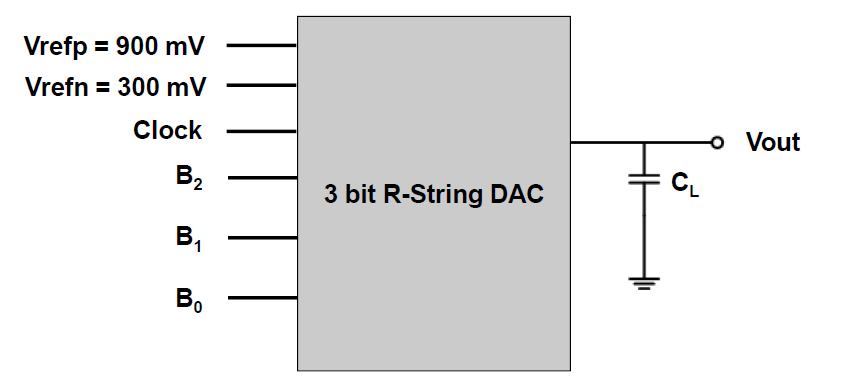
\includegraphics[scale=.5]{dac_task}
		\caption{3-bit Resistor String Digital-to-Analog Converter (DAC)}
		\label{fig:dac_task}
	\end{center}
\end{figure}

Furthermore some assistance was given regarding transistor lengths, mismatch analysis and design recommendations for the resistor string. The rest of the design had to be developed by each group and is discussed in the following sections.

\chapter{Resistor String}

The voltage references for the output of DAC are generated with help of resistor divider network. As it is a three bit DAC there will be eight different output voltage levels hence we require a divider network of resistors followed by an Analog Multiplexer. 

The resistor resistor value in the string is decided by taking into design constraints such as power dissipation, area, mismatch variations, speed and the value itself in comparison with ON and OFF state resistance of the transmission gates. 

The resistance used is a RNHR1000MML130E block from the UMC 130 library with a width of $\unit[2]{\mu m}$ and a length of $\unit[13]{\mu m}$. This results in a value of $\unit[6.3946]{k\Omega}$. The reason behind selecting this value is to minimize mismatch which 0.018, optimized area, power dissipation in specified limits and the value of the resistance is lower than the OFF resistance of the transmission gates. 

We have selected the second layout from the suggestion because it shows good results in comparison with the two other suggested layouts in terms of INL, DNL errors and offset. Also the number of resistors for the third, potentially more robust layout, is higher which results in a much larger area as compared to the second, chosen, layout. The improvements in error measurements and performance are also negligible. 

The resistor string layout is shown in figure \ref{fig:resstring} and results of resistor string are discussed in Integration section.

\begin{figure}[H]
     \begin{center}
        \subfigure[Schematic of Resistor String]{
            \label{fig:resstring_schematic}
           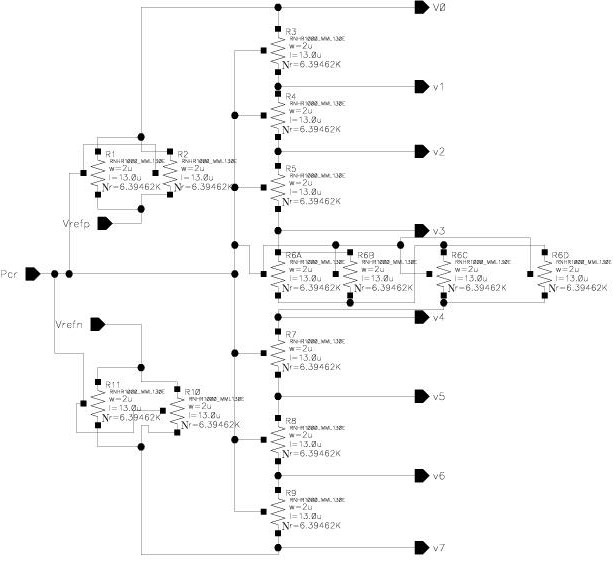
\includegraphics[scale=0.4]{Res_string2_schematic}
        }
        \subfigure[Layout of Resistor String]{
            \label{fig:resstring_layout}
            \includegraphics[scale=0.36]{Res_string2_layout2}
       }
       \caption{Schematic (a) and Layout (b) of resistor string.}
       \label{fig:resstring}
    \end{center}
\end{figure}

\chapter{Control Logic}

The Control Logic block in the DAC is used to generate clock synchronous select line signals.

\section{Components}

The basic building blocks of the Control Logic are inverters and transmission gates which form three D-Flip Flops.

\subsection{Inverter}

The Inverter is used to generate the inverted version of its input. The CMOS inverter consists of two transistors from the UMC 130 library: NMOS \texttt{N12HSL130E} and PMOS \texttt{P12HSL130E} as shown in figure \ref{fig:inverter}. 

\begin{figure}[H]
     \begin{center}
        \subfigure[Schematic of Inverter]{
            \label{fig:inverter_schematic}
           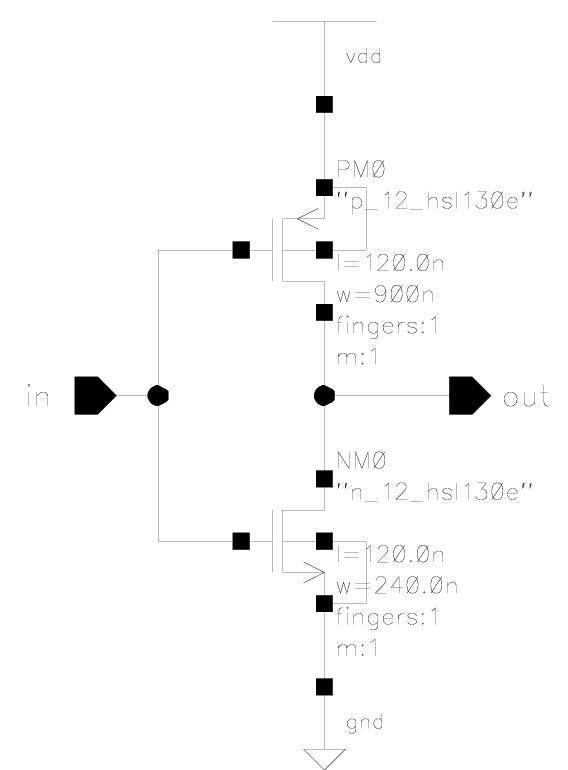
\includegraphics[scale=0.25]{Inverter_schematic}
        }
        \subfigure[Output of Simulation of Inverter]{
            \label{fig:inverter_sim}
         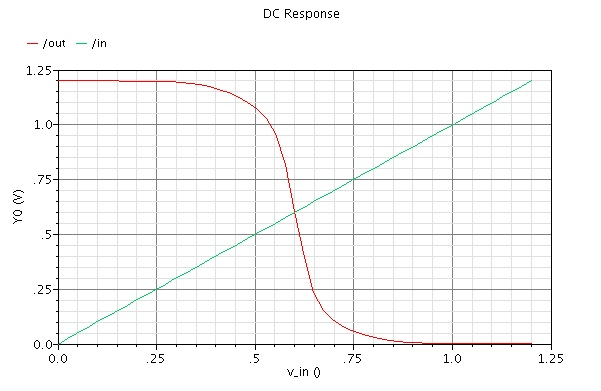
\includegraphics[scale=0.65]{Inverter_testbench_output}
        }
        \subfigure[Layout of Inverter]{
           \label{fig:inverter_layout}
           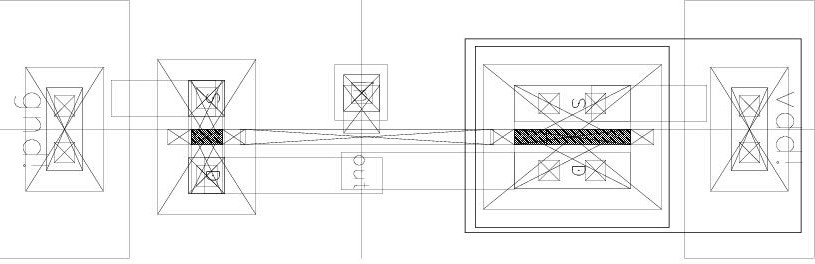
\includegraphics[scale=0.35]{Inverter_layout2}
        }   
       \caption{Schematic (a), DC Simulation (b) and Layout (c) of the designed inverter.}
       \label{fig:inverter}
    \end{center}
\end{figure}

The sizes of transistors are chosen to perform fast yet not too large so that the chip area and size of following circuit based on inverter remains minimum.

The Layout shown in above figure is the simplest as not many transistor are involved i.e. just PMOS and NMOS are placed side by side, input and output connection are made symmetrical by placing them in between and along with VDD and GND connection.

\subsection{Transmission Gate}


\begin{minipage}[t]{0.40\textwidth}
	\setlength{\parskip}{\currentparskip} % restore the value
The Transmission Gate also recognized as switch, is used to control the flow of signals through it with help of a control signal. Again, CMOS logic is used for transmission gates since by using both PMOS and NMOS transistors the disadvantage of each other are overcome to get better performance which is suitable for our design like keeping less ON state resistance for less power dissipation and less drop out voltage and high input resistance in OFF state. 

CMOS based design of transmission gate is shown in figure \ref{fig:txgate_schematic}. The same transistors and W/L ratios as for the inverter were used for the transmission gate, because the ratio of major charge carriers mobility is still the same. 
\end{minipage}
\begin{minipage}[t]{0.55\textwidth}
	\begin{figure}[H]
		\begin{center}
	        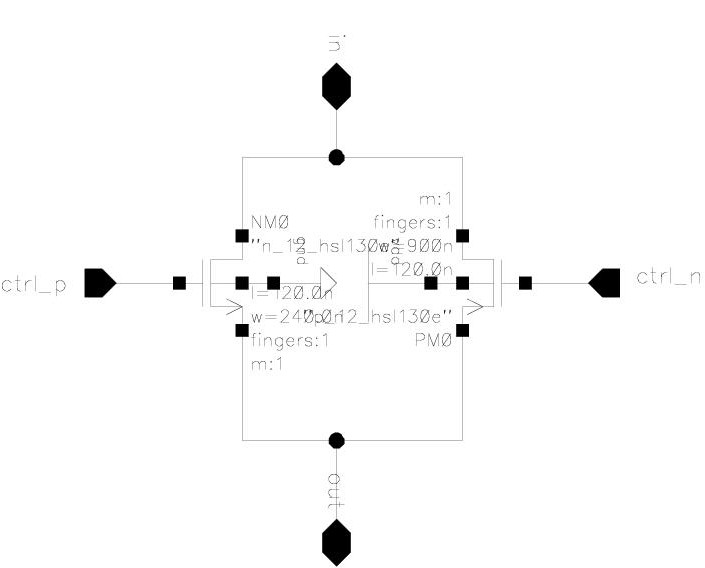
\includegraphics[scale=0.3]{Transmission_gate_schematic}
			\caption{Schematic of Transmission Gate}
            \label{fig:txgate_schematic}
		\end{center}			
	\end{figure}
\end{minipage}

The Layout of the transmission gate is shown in figure \ref{fig:txgate_layout}. Ground and power rails, as well as in- and output pins use the same grid layout as for the inverter layout cell.

\begin{figure}[H]
     \begin{center}
        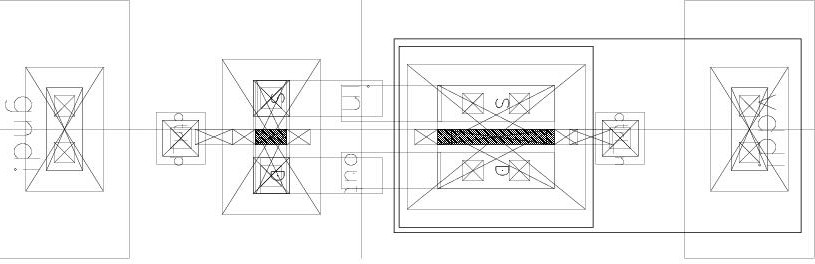
\includegraphics[scale=0.35]{Transmission_gate_layout2}
        \caption{Layout of Transmission Gate}
        \label{fig:txgate_layout}
    \end{center}
\end{figure}

\begin{minipage}[t]{0.35\textwidth}
	\setlength{\parskip}{\currentparskip} % restore the value
	For usage in analog circuitry like later discussed Analog Multiplexer (see chapter \ref{sec:analog_mux}), the \texttt{ON}- and \texttt{OFF-}state resistance is an important property of switch implementations.
	
	Figure \ref{fig:txgate_res} shows the simulation results for these two properties. The \texttt{OFF} state resistance of the designed transmission gate is at around $\unit[2]{G\Omega}$ to $\unit[3]{G\Omega}$. The \texttt{ON} state resistance of the designed transmission gate is at around $\unit[2]{k\Omega}$ to $\unit[3]{k\Omega}$. 
\end{minipage}
\begin{minipage}[t]{0.55\textwidth}
\begin{figure}[H]
     \begin{center}
         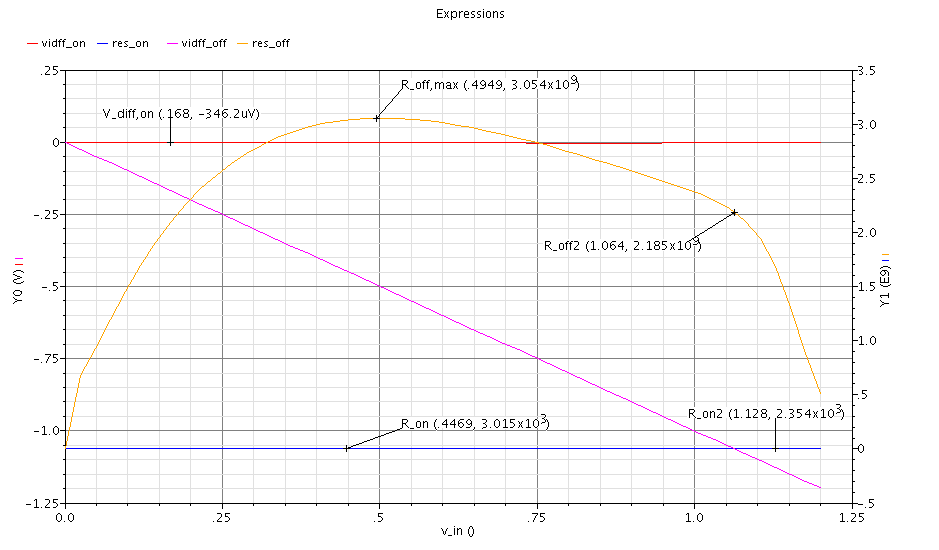
\includegraphics[scale=0.35]{txgate_res}
         \caption{Output of Simulation of Transmission Gate}
         \label{fig:txgate_res}
    \end{center}
\end{figure}
\end{minipage}

\subsection{D Flip-Flop}

The D Flip-Flop is designed in 2 stages containing inverters and transmission gates. The design uses minimum transistor i.e. 16 as compared to AND gate based logic design also other advantage of avoiding race condition and toggling. It has data \texttt{IN} (d) and positive (q) and negative (q\_n) \texttt{OUT}, as well as positive and negative clock signal ports. The output is available at positive clock edge. 

In design of D Flip-Flop two different inverters are used in different stages. In first stage the inverter with minimum area is selected with a W/L ratio large enough to drive only few gate. But the W/L ratio of the Inverters in second stage are large as compared to first one along with area to pass necessary current to drive large number of outputs which will be used in control logic to generate control signals for pass transistors. 

The schematic and layout of D Flip-Flop is shown in figure \ref{fig:dff}. 

\begin{figure}[H]
     \begin{center}
        \subfigure[Schematic of D Flip-Flop]{%
            \label{fig:dff_schematic}
          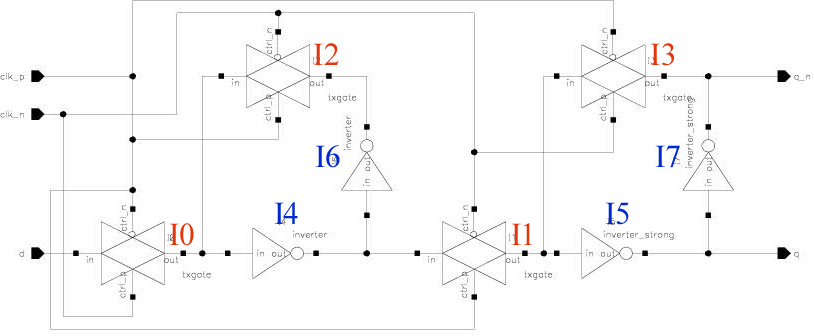
\includegraphics[scale=0.5]{DFlip-Flop_schematic3}
        }\\
        \subfigure[Layout of D Flip-Flop]{%
           \label{fig:dff_layout}
          \includegraphics[scale=0.5]{DFlip-Flop_layout3}
        }
        \caption{D Flip-Flop schematic (a), layout (b).}
        \label{fig:dff}
    \end{center}
\end{figure}

Inverter and transmission gate layout cells have a fixed height, therefore they can be composed to cells in an area efficient grid layout. All data in and out ports are on the same level which allows straight connections between neighboring cells.

Figure \ref{fig:dff_sim} show the simulation results for the designed D Flip-Flop with a simulated capacitive load of $\unit[10]{pF}$. Two key properties of the D Flip-Flop are visible in the graph: the Flip-Flop is capable to drive a large capacitive load and the output changes only at positive edges of the clock.

\begin{figure}[H]
	\begin{center}
		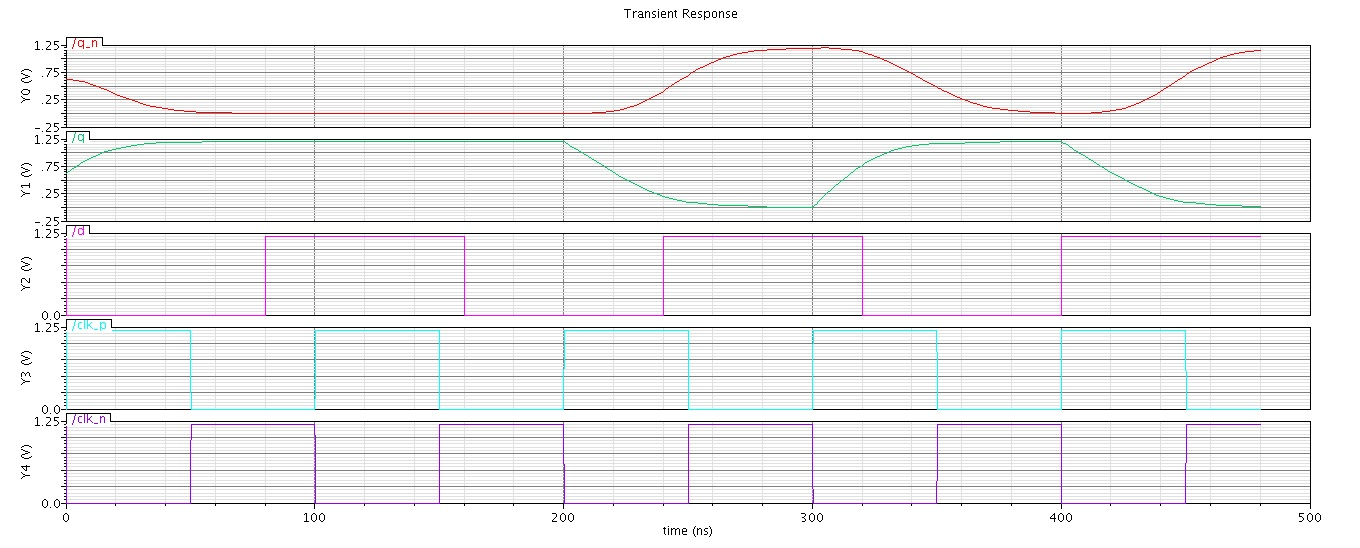
\includegraphics[scale=0.50]{DFlip-Flop_testbench_output}
        \caption{Output of Simulation of D Flip-Flop}
        \label{fig:dff_sim}	
	\end{center}
\end{figure}

The working of D Flip-Flop can be explained with help of following figure \ref{fig:dff_explanation}.

When the clock signal is high, the active path becomes 1-2-3-4-1 and 2-5-6-7-8 and when the clock signal is low, the active path is D-1-2-3-4. The second stage saves this state till next clock cycle using feedback path to maintain logic level at output.

\begin{figure}[H]
     \begin{center}
        \subfigure[Positive clock signal]{
            \label{fig:dff_explanation_1}
            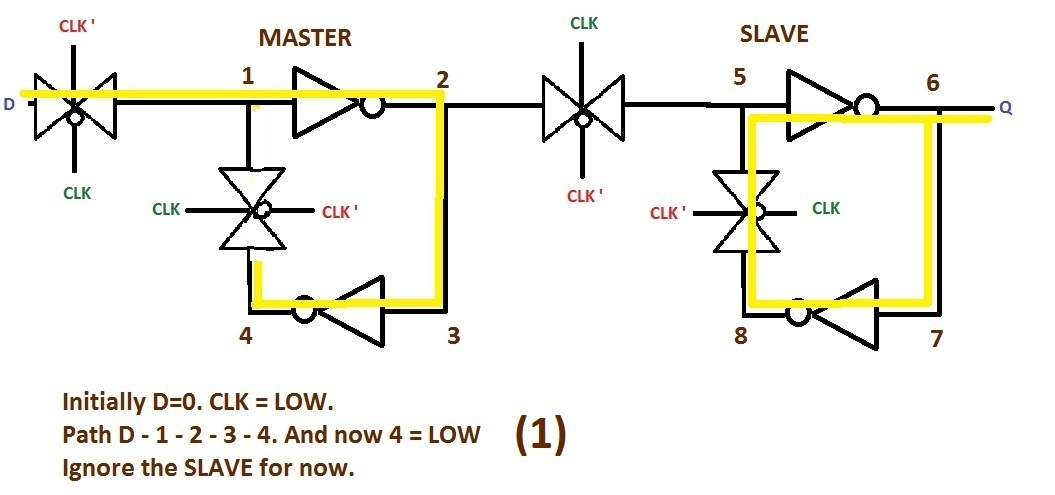
\includegraphics[width=0.45\linewidth]{Inverter_work}
        }
		\subfigure[Negative clock signal]{
            \label{fig:dff_explanation_2}
        	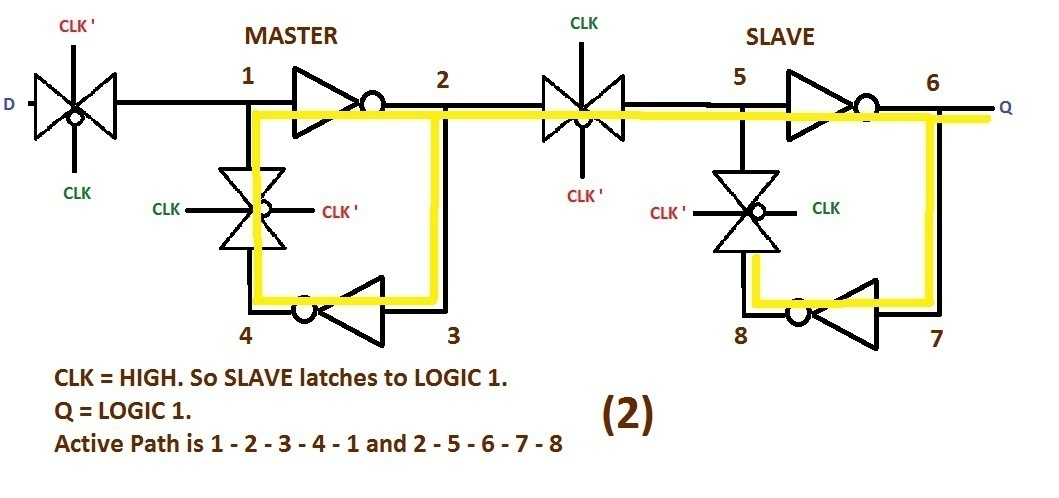
\includegraphics[width=0.45\linewidth]{Inverter_work2}       
        }
        \caption{Transmission gate D Flip-Flop.}
        \label{fig:dff_explanation}
    \end{center}
\end{figure}

\clearpage
\section{Top Level Control Logic Block}

The Control Logic is designed to generate the clocked synchronous buffered output signals along with there inverted versions of 3 input signals. \texttt{Clock}, \texttt{B0}, \texttt{B1} and \texttt{B2} are input signals and \texttt{Sel0}, \texttt{Sel0N}, \texttt{Sel1}, \texttt{Sel1N}, \texttt{Sel2}, \texttt{Sel2N} are output signals of the control logic block. The inverted clock required for the three D Flip-Flops is generated inside of the control logic block using a dedicated inverter.

Figure \ref{fig:ctrl_top} shows schematic and layout of the control logic block.

\begin{figure}[H]
     \begin{center}
        \subfigure[]{
            \label{fig:ctrl_top_schematic}
            \includegraphics[scale=0.5]{Control_schematic}
        }\\
        \subfigure[]{
            \label{fig:ctrl_top_layout}
         \includegraphics[scale=0.5]{Control_layout_fin}
        }
        \caption{Schematic (a) and layout (b) of the Control Logic block.}
        \label{fig:ctrl_top}
    \end{center}
\end{figure}


Figure \ref{fig:ctrl_propdelay} show the propagation time of the control logic block. The propagation time for rising signals is $T_\text{prop,rise} = \unit[159]{ps}$	and the propagation time for falling signals is $T_\text{prop,fall} = \unit[298]{ps}$. This would allow a clock frequency of about $\unit[3]{GHz}$ but examines only the control logic block and ignores additional timing constraints, like e.g. a setup and hold time for the flip flops.
\begin{figure}[H]
     \begin{center}
         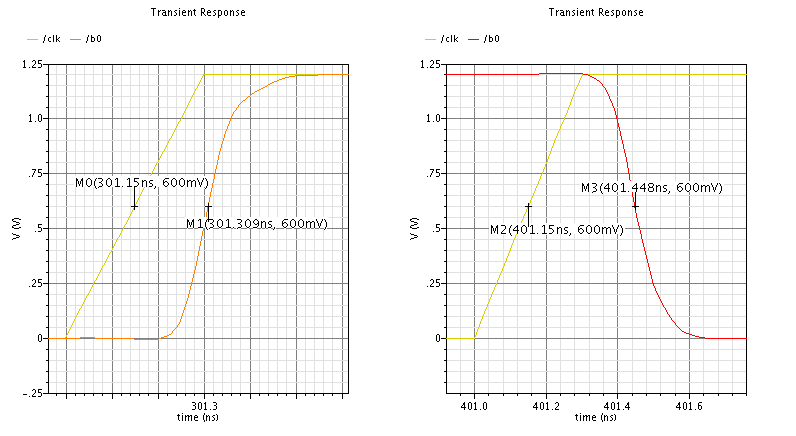
\includegraphics[scale=0.5]{ctrl_propdelay}
         \caption{Propagation time off control logic block (post layout).}
         \label{fig:ctrl_propdelay}
    \end{center}
\end{figure}

\chapter{Analog Multiplexer}
\label{sec:analog_mux}

The Analog Multiplexer consists of a number of cascaded transmission gates. The control signals i.e. \texttt{Sel0}, \texttt{Sel0N}, \texttt{Sel1}, \texttt{Sel1N}, \texttt{Sel2}, \texttt{Sel2N} generated by control logic block are used by these transmission gates. Depending upon this select signals a particular signal voltage is allowed to pass through this Multiplexer and at a time signal is pass through three pass transistor with a very less drop in voltage also shown in simulation results. 

The Schematic and Layout are shown in figure \ref{fig:analog_mux}. The layout is symmetrical with consecutive stages placed next to each other. Thereby only short connections are required, decreasing the routing complexity.

\begin{figure}[H]
     \begin{center}
        \subfigure[]{
            \label{fig:first}
          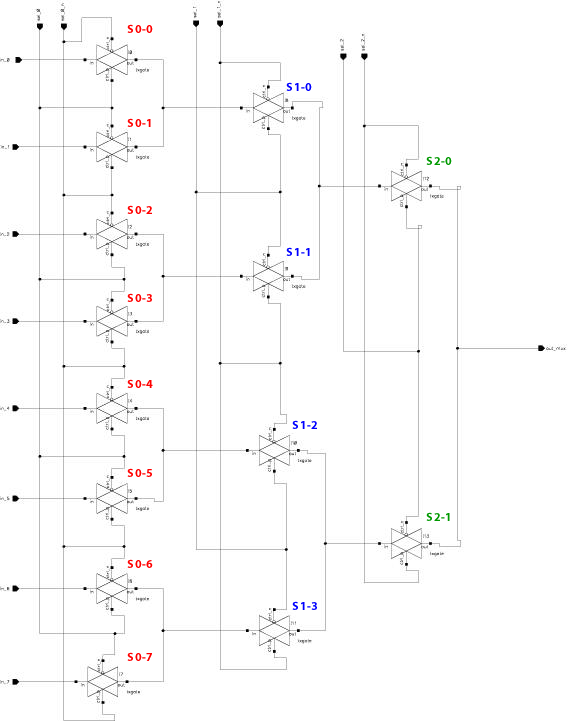
\includegraphics[scale=0.35]{Mux_schematic_fin}
        }
        \subfigure[]{
           \label{fig:second}
          \includegraphics[scale=0.36]{Mux_layout2_fin}
        }\\
        \subfigure[]{
            \label{fig:fourth}
            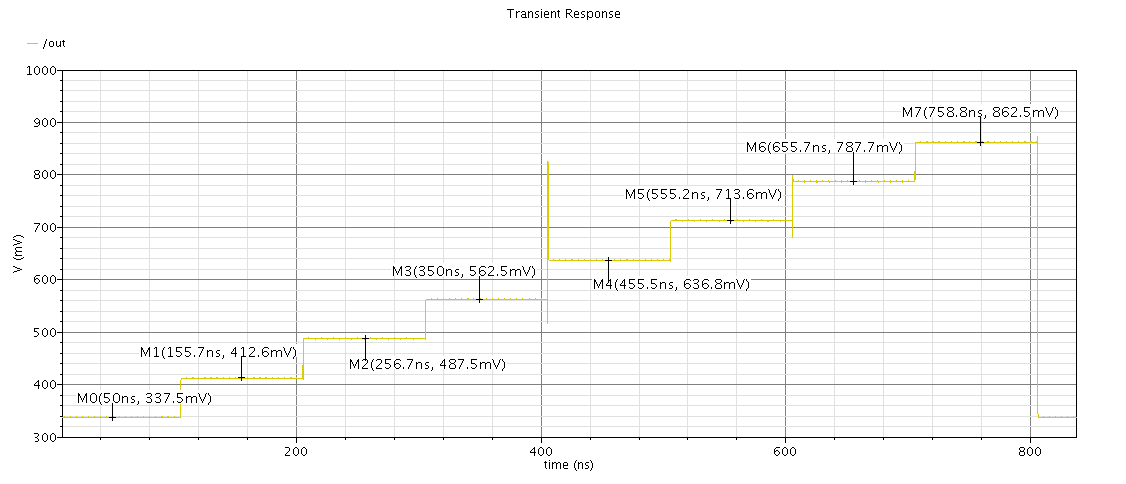
\includegraphics[scale=0.4]{mux_sim}
        }
        \caption{Schematic (a), layout (b) and simulation results (c) of analog multiplexer block.} 
        \label{fig:analog_mux}
    \end{center}
\end{figure}


\chapter{The Operational Amplifier}

\section{Calculation and Sizing of Transistors}

For the given schematic of the operational amplifier block, hand calculations were performed using the formulas from P. E. Allen\footnote{Dr. Phillip E. Allen: \glqq LECTURE 230 – DESIGN OF TWO-STAGE OP AMPS\grqq, \url{http://www.aicdesign.org/SCNOTES/2010notes/Lect2UP230\_\%28100327\%29.pdf} [07/2014]}.

The operational amplifier is designed for a load capacitance of $\unit[4]{pF}$. The coupling capacitance ($C_C$) was set to $C_C = 0.5 \cdot C_L = \unit[2]{pF}$, whereas the recommended formula for a phase margin of $60^\circ$ is $C_C \geq 0.22 \cdot C_L$. This change leads to an improved frequency stability.

For the first iteration of (hand) calculations the other specifications were taken as provided in the lab task. Variations in transistor threshold voltages were calculated using $V_\text{T0,min} = 0.8 \cdot V_\text{T0}$ and $V_\text{T0,max} = 1.2 \cdot V_\text{T0}$. The transistor lengths were chosen according to the provided material (design/implementation guidelines) for the lab (see table \ref{tab:opamp:wl}). 

Characteristics of the operational amplifier designed according to the described calculations did not meet all of the requirements. Therefore the input parameters (list of requirements) to the set of calculations were changed until all requirements were met. These changes to the parameters covered the \textit{Gain Bandwidth (GB)} and \textit{Slew Rate (SR)} requirements, which were finally set to $\text{GB} = \unit[200]{MHz}$ and $\text{SR} = \unit[30]{V/\mu s}$. The final transistor sizes are shown in table \ref{tab:opamp:wl}, column: \glqq Schematic without Mismatch\grqq.

\begin{table}[H]
  \centering
    \begin{tabular}{|r|r|r|r|r|r|r|}
    \hline
    \multicolumn{1}{|c|}{\multirow{2}[4]{*}{\textbf{Transistor}}} & \multicolumn{3}{c|}{\textbf{Hand calculations}} & \multicolumn{3}{c|}{\textbf{Schematic  without mismatch}}  \\
    \cline{2-7} \multicolumn{1}{|c|}{} & \textbf{W/L} & \textbf{W/µm} & \textbf{L/µm} & \multicolumn{1}{c|}{\textbf{W/L}} & \multicolumn{1}{c|}{\textbf{W/µm}} & \multicolumn{1}{c|}{\textbf{L/µm}} \\
    \hline
    \textbf{M1, M2} &  0.102  &  0.024  &  0.240  & 5.092 & 1.222 & 0.240 \\
    \hline
    \textbf{M3, M4} &  6.935  &  0.024  &  0.240  & 13.871 & 6.658 & 0.480 \\
    \hline
    \textbf{M5} &  2.865  &  3.329  &  0.480  & 5.731 & 2.063 & 0.360 \\
    \hline
    \textbf{M6} &  15.927  &  3.329  &  0.480  & 159.271 & 38.225 & 0.240 \\
    \hline
    \textbf{M7} &  3.290  &  0.790  &  0.240  & 32.900 & 7.896 & 0.240 \\
    \hline
    \textbf{M8} &  4.167 & 1.500  &  0.360  & 4.167 & 1.500 & 0.360 \\
    \hline
    \textbf{M9} &  16.667 & 2.000  &  0.120  & 16.667 & 2.000 & 0.120 \\
    \hline
    \textbf{$C_C$} & 2 pF &    &    & \multicolumn{1}{c|}{2 pF} & \multicolumn{1}{c|}{} & \multicolumn{1}{c|}{} \\
    \hline
    \end{tabular}
  \caption{W/L ratios of transistors in the opamp block}
  \label{tab:opamp:wl}
\end{table}

\subsection{Biasing Transistors M8 and M9}

The W/L ratio for transistor M8 was calculated using the formula $S_8 = I_8 \cdot \frac{S_5}{I_5}$ (with $S_i = \frac{W_i}{L_i}$), which is valid for current mirrors in general. The recommended value for $L_8$ was specified as $\unit[0.360]{\mu m}$. Therefore $W_8$ was set to $\unit[1.5]{\mu m}$.

Kirchhoff's current law demands $I_9 = I_8$, but $M_9$ is not part of the current mirror. Therefore $L_9$ was set to the minimum value of $\unit[0.120]{\mu m}$ to save chip area. This yields $W_9 = \unit[2.0]{\mu m}$.

\section{Simulation and Results}

A set of testbenches were created to simulate and characterize the designed operational amplifier. The results of all the simulations are specified in table \ref{tab:opamp_results}.

\begin{figure}[H]
	\begin{minipage}[t]{0.4\textwidth} 
	\setlength{\parskip}{\currentparskip} % restore the value
	\vspace{.3cm}
		The first testbench contains the operational amplifier with feedback loop and a DC sweep over the complete $V_\text{DD}$ range from $\unit[0]{V}$ to $\unit[1.2]{V}$ ($\unit[-600]{mV}$ to $\unit[+600]{mV}$ respectively). The result is shown in figure \ref{fig:opamp_sim1}. 
		
		From this simulation the input voltage range of the operational amplifier can be specified. As seen in the graph, the operational amplifier can operate with an input signal in the range from $\unit[81.5]{mV}$ to $\unit[993]{mV}$. There is almost no difference between pre-layout (schematic) and post-layout simulations for the input voltage range.
	\end{minipage}
	\begin{minipage}[t]{0.55\textwidth} 
		\begin{center}
			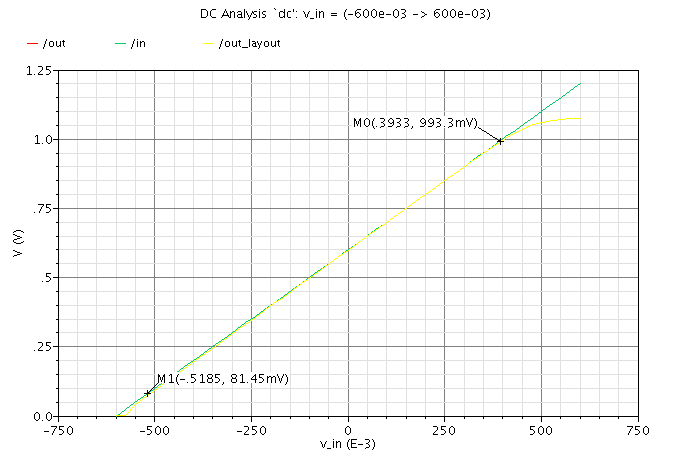
\includegraphics[scale=0.4]{opamp_sim1}
		    \caption{OpAmp simulation for input range specification.}
		    \label{fig:opamp_sim1}		
		\end{center}
	\end{minipage}
\end{figure}

\begin{figure}[H]
	\begin{minipage}[t]{0.55\textwidth} 
		\begin{center}
		    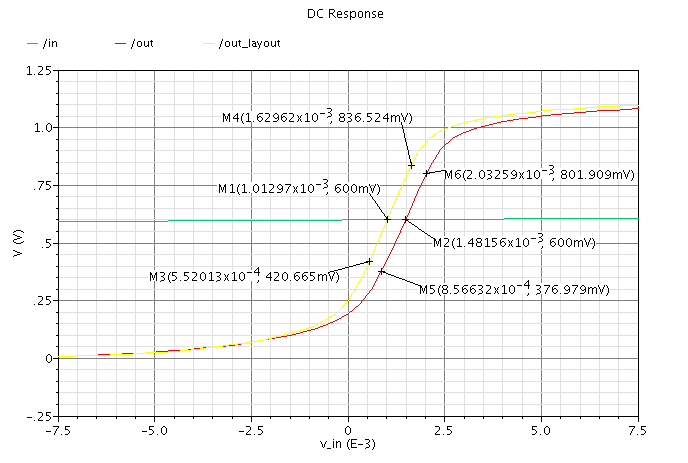
\includegraphics[scale=0.4]{opamp_openloop_detail}
		    \caption{Open loop OpAmp simulation.}
		    \label{fig:opamp_openloop_detail}	
		\end{center}
	\end{minipage}
	\begin{minipage}[t]{0.4\textwidth} 
	\setlength{\parskip}{\currentparskip} % restore the value
	\vspace{.8cm}
The DC gain characteristic can be specified using an open loop simulation. The output graph for this simulation is show in figure \ref{fig:opamp_openloop_detail}. 
The DC gain in dB can be calculated using the formula $A = 20 \cdot \log_{10} \left( \cfrac{V_\text{out2}-V_\text{out1}}{V_\text{in2}-V_\text{in1}} \right)$. 

The graph also shows the DC offset voltage of the amplifier (markers M1 and M2). This characteristic is important for further simulations.
 Another characteristic of the operational amplifier is the output voltage range which is also measured using an open loop simulation, but with a wider input voltage range. The output voltage range is specified in table \ref{tab:opamp_results}, but not shown in figure \ref{fig:opamp_openloop_detail}.
	\end{minipage}
\end{figure}

A third testbench was used to specify phase margin and bandwidth of the operational amplifier. This simulation consists of an AC sweep over the complete frequency range with an open loop configuration of the operational amplifier. For this this simulation it is important to compensate the DC offset of the amplifier using a DC voltage source in the testbench circuitry. A sinus with $\unit[+/-500]{mV}$ magnitude was used as input signal.

Figure \ref{fig:opamp_pm} show the results of this AC simulation. The unity gain frequencies are marked in the lower graph. The phase margin is specified as $\text{PM} = 180^\circ - \phi_\text{Vo,unity}$ with $\phi_\text{Vo,unity}$ as the phase of $V_\text{out}$ at unity gain frequency. As shown in the graphs results for pre-layout (schematic) and post-layout simulations vary only slightly but noticeable.

\begin{figure}[H]
	\begin{center}
		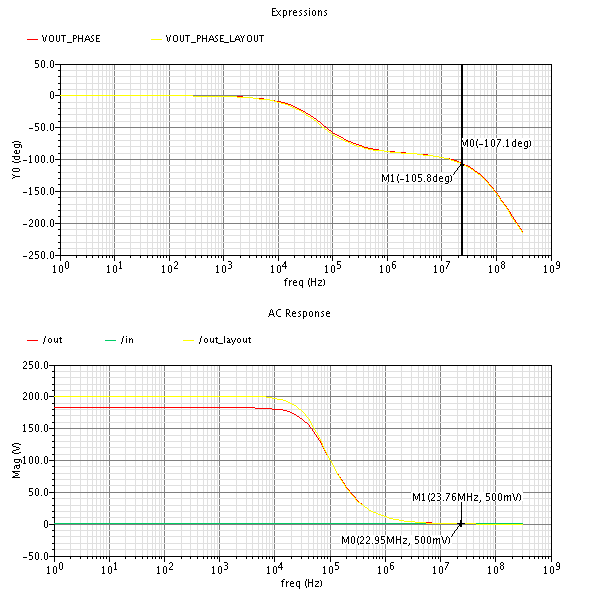
\includegraphics[scale=0.60]{opamp_pm}
	    \caption{OpAmp simulation for bandwidth and phase margin specification.}
	    \label{fig:opamp_pm}		
	\end{center}
\end{figure}

To specify the slew rate, another testbench and simulation setup was created. In this case a transient simulation with an input signal containing a rising and a falling edge is required. Figure \ref{fig:opamp_sr} shows the result of this simulation. 

\begin{figure}[H]
	\begin{center}
		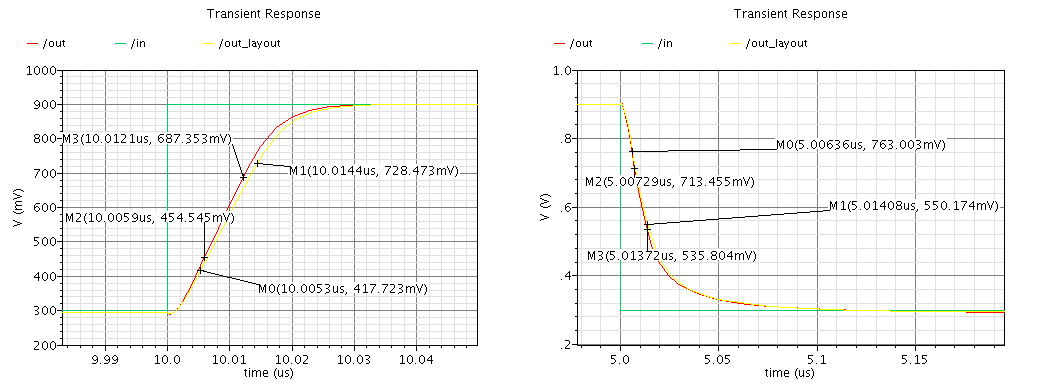
\includegraphics[width=\linewidth]{opamp_sr}
	    \caption{OpAmp simulation for slew rate (SR) specification.}
	    \label{fig:opamp_sr}
	\end{center}
\end{figure}

It is important to generate an input signal with a slew rate atleast as high as the required slew rate by the given specifications. This was missed during the initial simulations, because the default slew rate of the pulse generator voltage source in the \textit{Cadence Virtuouso} tool suite is $\unit[15]{V/ \mu s}$ and lead to over-engineering the strength of the operational amplifier while trying to meet the given specification. This example also shows that it is always important to understand the properties and limitations of the used testbench and to not blindly trust the results of simulations.

\begin{table}[H]
  \centering
    \begin{tabular}{|l|r|r|r|}
    \hline
    \textbf{Parameters} & \textbf{Required Specifications} & \textbf{Schematic Without Mismatch} & \textbf{Parasitic Extracted Layout} \\
    \hline
    DC Gain & > 50 dB & 50.91 dB & 51.73 dB \\
    \hline
    GB & > 20 MHz & 23.76 MHz & 23.76 MHz \\
    \hline
    PM & > 50° & 73.714° & 72.9° \\
    \hline
    SR & > 15 V/µs & 33 V/µs & 34 V/µs \\
    \hline
    $V_\text{in,min}$ & $\leq$ 300 mV & 81.5 mV & 81.5 mV  \\
    \hline
    $V_\text{in,max}$ & $\geq$ 900 mV & 993 mV & 993 mV \\
    \hline
    $V_\text{offset}$ & 0 mV & 1.482 mV & 1.013 mV \\
    \hline
    $V_\text{out,min}$ & $\leq$ 0.2 V & 0.00 V & 0.00 V \\
    \hline
    $V_\text{out,max}$ & $\geq$ 1.0 V & 1.14 V & 1.14 V \\
    \hline
    $P_\text{diss}$ & < 3 mW &  1.41 mW  & 1.239 mW \\
    \hline
    $C_L$ & > 1 pF & 4 pF & 4 pF \\
    \hline
    \end{tabular}%
  \caption{Simulation results for the operational amplifier}
  \label{tab:opamp_results}%
\end{table}%

\subsection{Mismatch}

The operational amplifier contains two (symmetrical) stages which need to be in perfect balance for best operation of the amplifier. This includes the differential stage with transistors M1 and M2 and the current mirror driving the differential stage consisting of transistors M3 and M4.

Due to properties of the fabrication process of the designed system, it must be assumed that these stages are not perfectly balanced, but contain slight differences in the transistor sizes. These variations were simulated on schematic level assuming $+/-\unit[30]{nm}$ difference in width for M2/M1 and M3/M4 respectively.

Simulation showed that the described variations in transistor sizes have almost no impact on slew rate, input and out voltage range, but are clearly visible in offset voltage and bandwidth and phase margin.

\begin{figure}[H]
     \begin{center}
        \subfigure[Open loop simulation with mismatch]{
            \label{fig:opamp_openloop_detail_mismatch}
          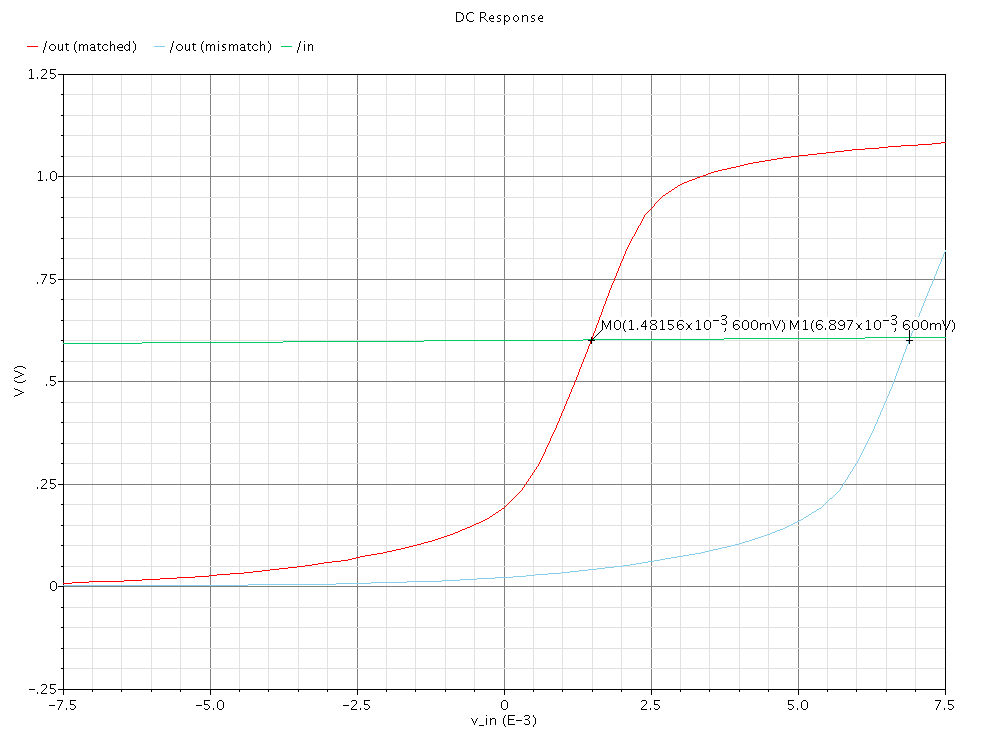
\includegraphics[width=0.47\linewidth]{opamp_openloop_detail_mismatch}
        }
        \subfigure[Bandwidth and phase margin simulation with mismatch]{
           \label{fig:opamp_pm_mismatch}
          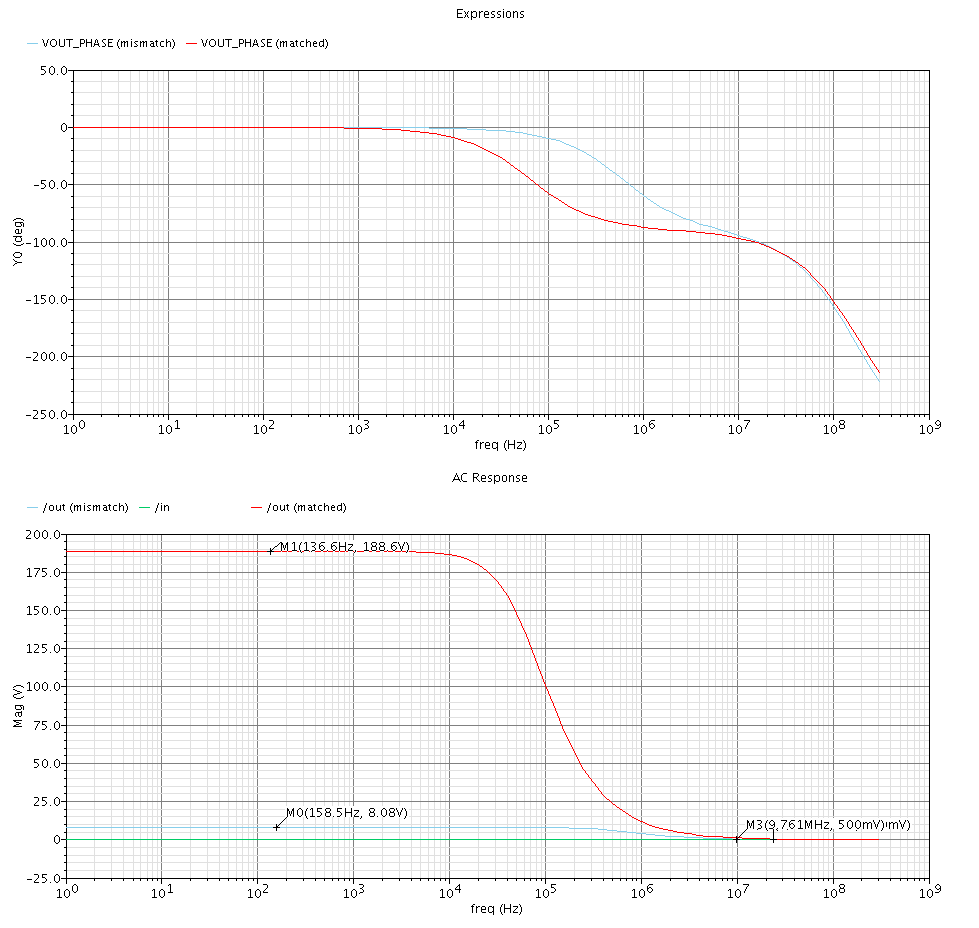
\includegraphics[width=0.40\linewidth]{opamp_pm_mismatch}
        }
    \end{center}
\end{figure}

\section{Layout}

The layout of the operational amplifier is shown in figure \ref{fig:opamp_layout}. The placement strategy for the operational amplifier was to position the transistors as in the schematic. This requires the placement of multiple N-Wells, but serves clarity.

\begin{figure}[H]
	\begin{center}
		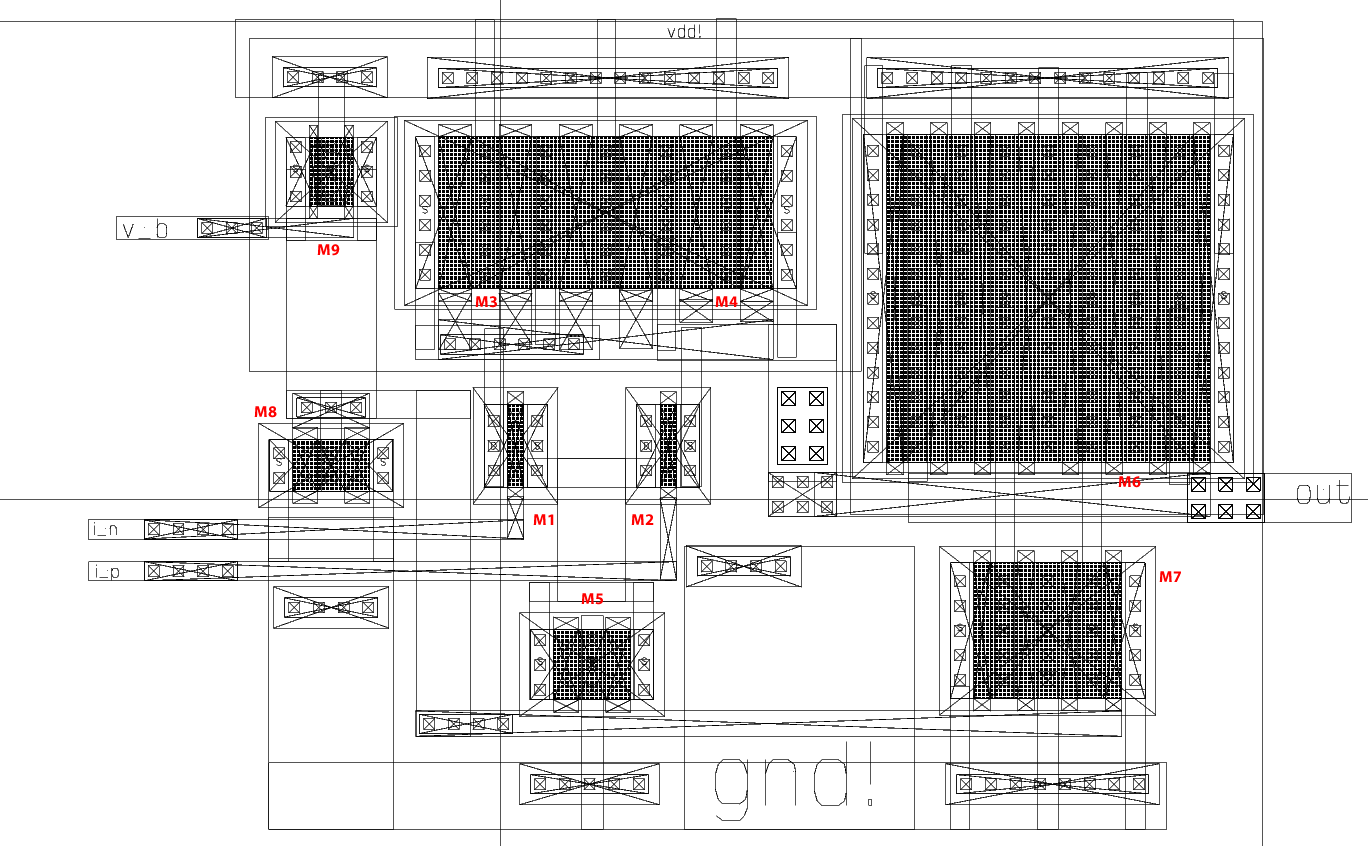
\includegraphics[width=\linewidth]{opanp_layout_fin}
	    \caption{OpAmp layout.}
	    \label{fig:opamp_layout}
	\end{center}
\end{figure}

\section{Reference Voltage}

\begin{wrapfigure}[10]{r}{.4\textwidth}
	\centering
    \includegraphics[scale=0.25]{v_ref_schem}
    \caption{Voltage divider}
    \label{fig:vrefschem}
\end{wrapfigure}

A simple voltage divider was implemented as reference voltage source for transistor M9 of the operational amplifier. For minimal mismatch between both resistors due to production inaccurances, the resistors should be in the range of $1.5\mu < W \leq 2.5\mu$ and $5\mu < L \leq 20\mu$. Therefore L was set to $1.5\mu$ and W was set to $14.94\mu$ for R0 and $12.71\mu$ for R1 (see figure \ref{fig:vrefschem}).

\begin{equation}
V_\text{ref} = 1.2 V \cdot \frac{9.957962 k\Omega}{9.957962 k\Omega + 8.426685 k\Omega} = 1.2 V \cdot 0.5416 = 649,97 mV
\end{equation}

\vspace{6cm}

\chapter{Digital-to-Analog Converter: Integration of Design Blocks}
All the blocks discussed previously are integrated in a single Digital to Analog Converter cell. The input to this whole block are three digital input bits \texttt{B0}, \texttt{B1}, \texttt{B2}, two reference voltage pins \texttt{Vrefp} and \texttt{Vrefn}, along with a clock signal and one output pin. 

The resistor string block uses the reference inputs voltages across its string to generate the necessary corresponding bit voltages. The output of the resistor string is connected to the analog multiplexer which feeds the OP-Amp block. The OP-Amp is used as buffer to drive the output load. 

The whole schematic is shown in figure \ref{fig:dac_schematic}.

\begin{figure}[H]
	\begin{center}
		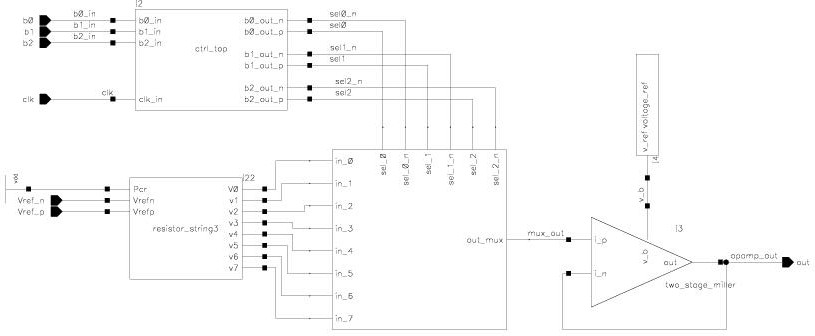
\includegraphics[scale=0.5]{top_schematic}
		 \caption{Schematic of the Digital-to-Analog converter.}
		 \label{fig:dac_schematic}
	\end{center}
\end{figure}

\section{Layout}

Figure \ref{fig:dac_layout} shows the overall Digital-to-Analog converter layout with highlighted component blocks. Three aspects were important for the placement of components: optimal area utilization, signal flow (input and output) from left to right, top to bottom and minimum analog signal paths.

\begin{figure}[H]
	\begin{center}
		\includegraphics[width=\linewidth]{top_layout2_fin}
		 \caption{Layout of the Digital-to-Analog converter.}
		 \label{fig:dac_layout}
	\end{center}
\end{figure}

The total area is $\unit[59]{\mu m} \text{ x } \unit[42]{\mu m}$ and primarily dictated by the size of coupling capacitor $C_C$. This capacitor is placed on top of all components and covers the whole area. A smaller layout size would only be possible with a smaller coupling capacitor. The whole DAC is designed for a load capacitance of $\unit[4]{pF}$. This is four times the required minimum load capacitance, therefore there would be still room for a reduction in area size.

\section{Simulations}

Figure \ref{fig:dac_out} shows the simulation results for the final output of the DAC. Based on this figures error characteristics can be calculated. These include offset, gain, DNL and INL error. All results are documented in table \ref{tab:dac_errors}.

The offset error at post layout simulation is $\unit[-0.054]{LSB}$, the gain error is $\unit[0.047]{LSB}$, the INL error varies between $\unit[0.013]{LSB}$ and $\unit[0.054]{LSB}$ (absolute values) and the DNL error varies between $\unit[0.002]{LSB}$ and $\unit[0.067]{LSB}$. All these figures are $\ll \unit[0.5]{LSB}$, therefore the specified quality requirement is met.

The following formulas were used to calculate the errors:

Offset error (in mV): $V_\text{err,offset} = V_\text{out,0} - \unit[337.5]{mV}$

Gain error (in mV): $V_\text{err,gain} = V_\text{out,7} - V_\text{err,gain} - \unit[862.5]{mV}$

Let $V_\text{out,norm,i} = \left( V_\text{out,i} - V_\text{err,offset} \right) \cdot \frac{\unit[862.5]{mV}}{V_\text{out,7}}$

INL error (in mV, for output $i$, with $i \in \left[ 0, 7 \right]$): $\text{INL}_i =  V_\text{out,norm,i} - \unit[337.5]{mV} - i \cdot \unit[75]{mV}$

DNL error (in mV, for output $i$, with $i \in \left[ 0, 6 \right]$): $\text{DNL}_i =  V_\text{out,norm,i+1} - V_\text{out,norm,i} - \unit[75]{mV}$

\begin{figure}[H]
	\begin{center}
		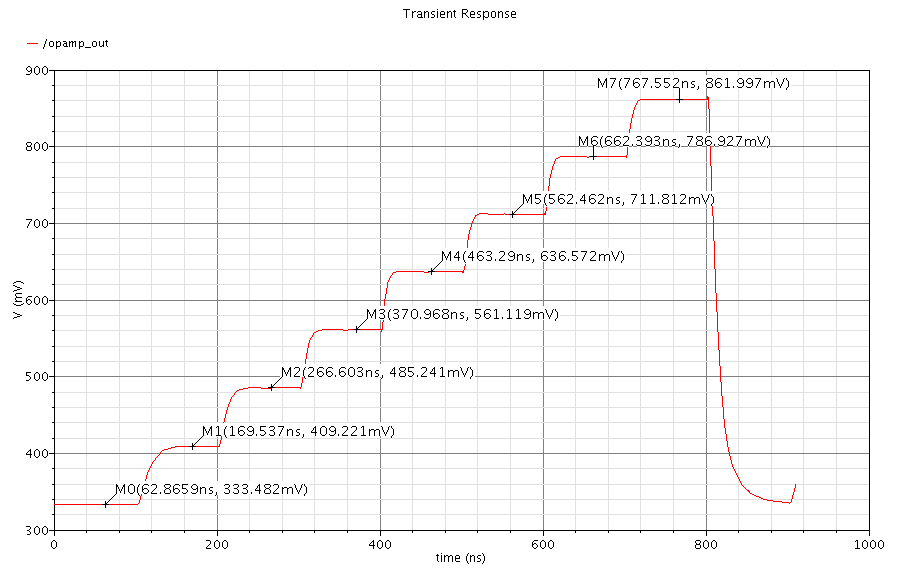
\includegraphics[width=\linewidth]{dac_out}
		 \caption{Simulation results with Digital-to-Analog converter output voltages (post layout).}
		 \label{fig:dac_out}
	\end{center}
\end{figure}

\begin{sidewaystable}
\tiny
  \centering
    \begin{tabular}{|r|r|r|r|r|r|r|r|r|r|r|r|r|r|r|r|r|}
    \hline
\multicolumn{1}{|c|}{\textbf{Bits}} & \multicolumn{2}{c|}{\textbf{Without Mismatch}} & \multicolumn{2}{c}{\textbf{Mismatch case 1a}} & \multicolumn{2}{c|}{\textbf{Mismatch case 1b}} & \multicolumn{2}{c}{\textbf{Mismatch Case 2a}} & \multicolumn{2}{c|}{\textbf{Mismatch case 2b}} & \multicolumn{2}{c}{\textbf{Mismatch case 3a}} & \multicolumn{2}{c|}{\textbf{Mismatch case 3b}} & \multicolumn{2}{c|}{\textbf{Parasitic Extracted Layout}} \\
    \textbf{} & \multicolumn{2}{c|}{\textbf{}} & \multicolumn{2}{c}{\textbf{Res\_Min}} & \multicolumn{2}{c|}{\textbf{Res\_Max}} & \multicolumn{2}{c}{\textbf{Res\_Min}} & \multicolumn{2}{c|}{\textbf{Res\_Max}} & \multicolumn{2}{c}{\textbf{Res\_Min}} & \multicolumn{2}{c|}{\textbf{Res\_Max}} & \multicolumn{1}{r}{\textbf{}} & \textbf{} \\
    \hline
    \textbf{Power / mW} & \multicolumn{2}{c|}{0.7870} & \multicolumn{2}{c|}{0.7929} & \multicolumn{2}{c|}{} & \multicolumn{2}{c|}{} & \multicolumn{2}{c|}{} & \multicolumn{2}{c|}{0.7950} & \multicolumn{2}{c|}{0.7903} & \multicolumn{2}{c|}{0.7069} \\
    \hline
    \textbf{Offset} & -0.032 & -2.4 & -0.019 & -1.4 & 0.005 & 0.4 & -0.017 & -1.3 & -0.013 & -1 & -0.017 & -1.3 & -0.036 & -2.7 & -0.054 & -4.018 \\
    \hline
    \textbf{Gain} & 0.020 & 1.5 & 0.005 & 0.4 & -0.017 & -1.3 & 0.003 & 0.2 & 0.003 & 0.2 & 0.137 & 10.3 & 0.020 & 1.5 & 0.047 & 3.515 \\
    \hline
 \multicolumn{1}{|r}{\textbf{Output}} & \multicolumn{1}{c}{\textbf{measured}} & \multicolumn{1}{c}{\textbf{w/o error}} & \multicolumn{1}{c}{\textbf{measured}} & \multicolumn{1}{c}{\textbf{w/o error}} & \multicolumn{1}{c}{\textbf{measured}} & \multicolumn{1}{c}{\textbf{w/o error}} & \multicolumn{1}{c}{\textbf{measured}} & \multicolumn{1}{c}{\textbf{w/o error}} & \multicolumn{1}{c}{\textbf{measured}} & \multicolumn{1}{c}{\textbf{w/o error}} & \multicolumn{1}{c}{\textbf{measured}} & \multicolumn{1}{c}{\textbf{w/o error}} & \multicolumn{1}{c}{\textbf{measured}} & \multicolumn{1}{c}{\textbf{w/o error}} & \multicolumn{1}{c}{\textbf{measured}} & \multicolumn{1}{c|}{\textbf{w/o error}} \\
    \hline
    \textbf{000 / mV} & 335.1 & 335.100 & 336.1 & 336.100 & 337.9 & 337.900 & 336.2 & 336.200 & 336.5 & 336.500 & 336.2 & 336.200 & 334.8 & 334.800 & 333.482 & 333.482 \\
    \hline
    \textbf{001 / mV} & 408.9 & 411.730 & 408.0 & 409.875 & 409.7 & 409.728 & 408.4 & 410.223 & 409.8 & 411.181 & 411.0 & 408.042 & 408.8 & 412.073 & 409.221 & 413.480 \\
    \hline
    \textbf{010 / mV} & 484.8 & 487.709 & 484.9 & 486.864 & 484.3 & 484.405 & 485.4 & 487.322 & 484.3 & 485.751 & 488.2 & 484.445 & 484.7 & 488.079 & 485.241 & 489.544 \\
    \hline
    \textbf{011 / mV} & 560.6 & 563.588 & 559.9 & 561.952 & 561.0 & 561.186 & 560.5 & 562.517 & 560.8 & 562.322 & 565.3 & 560.749 & 560.5 & 563.985 & 561.119 & 565.467 \\
    \hline
    \textbf{100 / mV} & 636.3 & 639.367 & 636.6 & 638.741 & 635.6 & 635.864 & 636.4 & 638.514 & 636.2 & 637.792 & 642.3 & 636.954 & 636.2 & 639.790 & 636.572 & 640.964 \\
    \hline
    \textbf{101 / mV} & 711.7 & 714.846 & 711.3 & 713.527 & 711.8 & 712.143 & 711.1 & 713.310 & 712.2 & 713.862 & 719.1 & 712.960 & 711.5 & 715.195 & 711.812 & 716.248 \\
    \hline
    \textbf{110 / mV} & 786.8 & 790.024 & 787.5 & 789.816 & 785.9 & 786.321 & 787.4 & 789.707 & 786.2 & 787.931 & 795.4 & 788.472 & 786.6 & 790.400 & 786.927 & 791.407 \\
    \hline
    \textbf{111 / mV} & 861.6 & 864.903 & 861.5 & 863.902 & 861.6 & 862.100 & 861.4 & 863.802 & 861.7 & 863.501 & 871.5 & 863.787 & 861.3 & 865.204 & 861.997 & 866.520 \\
    \hline
    \multicolumn{1}{|r}{\textbf{INL Errors}} & \multicolumn{1}{c}{\textbf{/ LSB}} & \multicolumn{1}{c}{\textbf{/ mV}} & \multicolumn{1}{c}{\textbf{/ LSB}} & \multicolumn{1}{c}{\textbf{/ mV}} & \multicolumn{1}{c}{\textbf{/ LSB}} & \multicolumn{1}{c}{\textbf{/ mV}} & \multicolumn{1}{c}{\textbf{/ LSB}} & \multicolumn{1}{c}{\textbf{/ mV}} & \multicolumn{1}{c}{\textbf{/ LSB}} & \multicolumn{1}{c}{\textbf{/ mV}} & \multicolumn{1}{c}{\textbf{/ LSB}} & \multicolumn{1}{c}{\textbf{/ mV}} & \multicolumn{1}{c}{\textbf{/ LSB}} & \multicolumn{1}{c}{\textbf{/ mV}} & \multicolumn{1}{c}{\textbf{/ LSB}} & \multicolumn{1}{c|}{\textbf{/ mV}} \\
    \hline
    \textbf{000} & -0.032 & -2.400 & -0.019 & -1.400 & 0.005 & 0.400 & -0.017 & -1.300 & -0.013 & -1.000 & -0.017 & -1.300 & -0.036 & -2.700 & -0.054 & -4.018 \\
    \hline
    \textbf{001} & -0.010 & -0.770 & -0.035 & -2.625 & -0.037 & -2.772 & -0.030 & -2.277 & -0.018 & -1.319 & -0.059 & -4.458 & -0.006 & -0.427 & 0.013 & 0.980 \\
    \hline
    \textbf{010} & 0.003 & 0.209 & -0.008 & -0.636 & -0.041 & -3.095 & -0.002 & -0.178 & -0.023 & -1.749 & -0.041 & -3.055 & 0.008 & 0.579 & 0.027 & 2.044 \\
    \hline
    \textbf{011} & 0.015 & 1.088 & -0.007 & -0.548 & -0.018 & -1.314 & 0.000 & 0.017 & -0.002 & -0.178 & -0.023 & -1.751 & 0.020 & 1.485 & 0.040 & 2.967 \\
    \hline
    \textbf{100} & 0.025 & 1.867 & 0.017 & 1.241 & -0.022 & -1.636 & 0.014 & 1.014 & 0.004 & 0.292 & -0.007 & -0.546 & 0.031 & 2.290 & 0.046 & 3.464 \\
    \hline
    \textbf{101} & 0.031 & 2.346 & 0.014 & 1.027 & -0.005 & -0.357 & 0.011 & 0.810 & 0.018 & 1.362 & 0.006 & 0.460 & 0.036 & 2.695 & 0.050 & 3.748 \\
    \hline
    \textbf{110} & 0.034 & 2.524 & 0.031 & 2.316 & -0.016 & -1.179 & 0.029 & 2.207 & 0.006 & 0.431 & 0.013 & 0.972 & 0.039 & 2.900 & 0.052 & 3.907 \\
    \hline
    \textbf{111} & 0.032 & 2.403 & 0.019 & 1.402 & -0.005 & -0.400 & 0.017 & 1.302 & 0.013 & 1.001 & 0.017 & 1.287 & 0.036 & 2.704 & 0.054 & 4.020 \\
    \hline
    \multicolumn{1}{|r}{\textbf{DNL Errors}} & \multicolumn{1}{c}{\textbf{/ LSB}} & \multicolumn{1}{c}{\textbf{/ mV}} & \multicolumn{1}{c}{\textbf{/ LSB}} & \multicolumn{1}{c}{\textbf{/ mV}} & \multicolumn{1}{c}{\textbf{/ LSB}} & \multicolumn{1}{c}{\textbf{/ mV}} & \multicolumn{1}{c}{\textbf{/ LSB}} & \multicolumn{1}{c}{\textbf{/ mV}} & \multicolumn{1}{c}{\textbf{/ LSB}} & \multicolumn{1}{c}{\textbf{/ mV}} & \multicolumn{1}{c}{\textbf{/ LSB}} & \multicolumn{1}{c}{\textbf{/ mV}} & \multicolumn{1}{c}{\textbf{/ LSB}} & \multicolumn{1}{c}{\textbf{/ mV}} & \multicolumn{1}{c}{\textbf{/ LSB}} & \multicolumn{1}{c|}{\textbf{/ mV}} \\
    \hline
    \textbf{000} & 0.022 & 1.630 & -0.016 & -1.225 & -0.042 & -3.172 & -0.013 & -0.977 & -0.004 & -0.319 & -0.042 & -3.158 & 0.030 & 2.273 & 0.067 & 4.998 \\
    \hline
    \textbf{001} & 0.013 & 0.979 & 0.027 & 1.989 & -0.004 & -0.322 & 0.028 & 2.098 & -0.006 & -0.431 & 0.019 & 1.403 & 0.013 & 1.006 & 0.014 & 1.064 \\
    \hline
    \textbf{010} & 0.012 & 0.879 & 0.001 & 0.087 & 0.024 & 1.780 & 0.003 & 0.196 & 0.021 & 1.571 & 0.017 & 1.304 & 0.012 & 0.906 & 0.012 & 0.922 \\
    \hline
    \textbf{011} & \multicolumn{1}{r}{0.010} & 0.779 & 0.024 & 1.789 & -0.004 & -0.322 & 0.013 & 0.997 & 0.006 & 0.470 & 0.016 & 1.205 & 0.011 & 0.805 & 0.007 & 0.497 \\
\cline{1-8}\cline{10-17}    \textbf{100} & 0.006 & 0.479 & -0.003 & -0.213 & 0.017 & 1.280 & -0.003 & -0.205 & 0.014 & 1.071 & 0.013 & 1.007 & 0.005 & 0.405 & 0.004 & 0.284 \\
    \hline
    \textbf{101} & 0.002 & 0.178 & 0.017 & 1.288 & -0.011 & -0.823 & 0.019 & 1.397 & -0.012 & -0.931 & 0.007 & 0.512 & 0.003 & 0.205 & 0.002 & 0.159 \\
    \hline
    \textbf{110} & -0.002 & -0.122 & -0.012 & -0.914 & 0.010 & 0.779 & -0.012 & -0.906 & 0.008 & 0.570 & 0.004 & 0.314 & -0.003 & -0.196 & 0.002 & 0.114 \\
    \hline
    \textbf{111} &    &    &    &    &    &    &    &    &    &    &    &    &    &    &    &  \\
    \hline
    \end{tabular}
  \caption{DAC simulation results with offset, gain, INL and DNL errors.}
  \label{tab:dac_errors}
\end{sidewaystable}

\end{document}
